\documentclass[aspectratio=169,11pt]{beamer}

\usepackage[utf8]{inputenc}
\usepackage[T1]{fontenc}
\usepackage{amsmath,amssymb,mathtools}
\usepackage{bm}
\usepackage{tikz}
\usetikzlibrary{backgrounds}
\usepackage{graphicx}
\usepackage{booktabs}
\usepackage{ragged2e}
\usepackage{microtype}
\usepackage[style=authoryear,backend=biber,dashed=false]{biblatex}
\addbibresource{refs.bib}

% ------------------------------------------------------------
% Palette
% ------------------------------------------------------------
\definecolor{PastelBlue}{HTML}{D4E6F1}
\definecolor{PureWhite}{HTML}{FFFFFF}
\definecolor{Navy}{HTML}{1F4E79}
\definecolor{Charcoal}{HTML}{2C3E50}
\definecolor{Peach}{HTML}{FADBD8}
\definecolor{Mustard}{HTML}{F7DC6F}

\usetheme{default}
\usefonttheme{professionalfonts}
\setbeamertemplate{navigation symbols}{}
\setbeamertemplate{headline}{}
\setbeamertemplate{footline}{%
  \begin{beamercolorbox}[wd=\paperwidth,ht=2.5ex,dp=1.3ex,leftskip=0.75cm,rightskip=0.75cm]{footline}
    \color{Navy}\scriptsize Learning Residual-Free Bubbles\hfill\insertframenumber/\inserttotalframenumber
  \end{beamercolorbox}}

\setbeamercolor{normal text}{fg=Charcoal,bg=PureWhite}
\setbeamercolor{frametitle}{fg=Navy,bg=PureWhite}
\setbeamercolor{title}{fg=Navy,bg=PureWhite}
\setbeamercolor{subtitle}{fg=Charcoal,bg=PureWhite}
\setbeamercolor{block title}{fg=Navy,bg=PastelBlue}
\setbeamercolor{block body}{fg=Charcoal,bg=PastelBlue!28!PureWhite}
\setbeamercolor{footline}{fg=Navy,bg=PureWhite}
\setbeamertemplate{itemize item}{\color{Navy}\small$\blacktriangleright$}
\setbeamertemplate{itemize subitem}{\color{Mustard}\tiny$\bullet$}

\setbeamerfont{title}{series=\bfseries,size=\Large}
\setbeamerfont{subtitle}{size=\normalsize}
\setbeamerfont{frametitle}{series=\bfseries,size=\large}
\setbeamerfont{block title}{series=\bfseries,size=\normalsize}

% ------------------------------------------------------------
% Helpers
% ------------------------------------------------------------
\newcommand{\accentbar}{%
\begin{tikzpicture}[remember picture,overlay]
  \fill[Peach] ([xshift=0.70cm,yshift=-0.86cm]current page.north west) rectangle ++(2.1cm,0.08cm);
  \fill[Mustard] ([xshift=2.95cm,yshift=-0.86cm]current page.north west) rectangle ++(0.85cm,0.08cm);
\end{tikzpicture}}

\newcommand{\softbox}[2]{%
\begin{tikzpicture}
\node[rounded corners=8pt, fill=#1, inner xsep=8pt, inner ysep=6pt, text width=0.88\linewidth, align=left] {#2};
\end{tikzpicture}}

\newcommand{\modelop}{\mathcal{L}}
\newcommand{\dd}{\,\mathrm{d}}
\newcommand{\Pe}{\operatorname{Pe}}
\newcommand{\KAN}{KAN}

\title{\Large Learning Residual-Free Bubbles\\
\large to Solve Elliptic Problems}
\author{Juan Felipe Pacazuca Santiago}
\date{}

\begin{document}

% ------------------------------------------------------------
\begin{frame}[plain]
\begin{tikzpicture}[remember picture,overlay]
  \fill[PastelBlue] (current page.south west) rectangle (current page.north east);
  \fill[PureWhite] ([xshift=0.65cm,yshift=0.65cm]current page.south west) rectangle ([xshift=-0.65cm,yshift=-0.65cm]current page.north east);
  \fill[Peach] ([xshift=0.95cm,yshift=-1.0cm]current page.north west) rectangle ++(2.0cm,0.12cm);
  \fill[Mustard] ([xshift=3.1cm,yshift=-1.0cm]current page.north west) rectangle ++(1.0cm,0.12cm);
\end{tikzpicture}
\vfill
\vfill\vfill
{\centering
{\color{Navy}\bfseries\LARGE Learning Residual-Free Bubbles}\\[0.1cm]
{\color{Charcoal}\large to Solve Elliptic Problems}\\[1.0cm]
\textbf{Juan Pacazuca Santiago}\\[0.3cm]
%\softbox{PastelBlue!45!PureWhite}{%
%\centering \textbf{Juan Pacazuca Santiago}}\\[0.3cm]
{\color{Navy}\small GA036 -- Introdução ao Aprendizado de Máquina}\par}
\vfill
\end{frame}

% ------------------------------------------------------------
\begin{frame}{1. The model}
\accentbar
We consider the one-dimensional reaction-advection-diffusion problem
\begin{equation*}
    -(\varepsilon u')' + \beta u' + \sigma u = f
    \quad\text{in }(0,\ell),
    \qquad
    u(0)=u(\ell)=0.
\end{equation*}

\vspace{0.2cm}
\softbox{PastelBlue!35!PureWhite}{%
\textbf{Weak form.} Find $u\in H_0^1(0,\ell)$ such that
\[
a(u,v)=L(v) \quad \forall v\in H_0^1(0,\ell),
\]
with
\[
\begin{aligned}
a(w,v)&=\int_0^\ell \varepsilon w'v' + \beta w'v + \sigma wv\,dx,\\
L(v)&=\int_0^\ell fv\,dx.
\end{aligned}
\]}
% \begin{columns}[T]
% \begin{column}{0.50\linewidth}

% \end{column}
% \begin{column}{0.44\linewidth}
% \softbox{Peach!55!PureWhite}{%
% When $Pe = \frac{\beta h}{\varepsilon} \gg 1$, the solution may contain a sharp boundary layer. Classical Galerkin on a coarse mesh can oscillate.}
% \end{column}
% \end{columns}
\end{frame}

% ------------------------------------------------------------
\begin{frame}{2. The Galerkin idea}
\accentbar
Let $V_h^1\subset H_0^1(0,\ell)$ be the continuous piecewise-linear finite element space.
\[
V_h^1 = \{v_1\in H_0^1(0,\ell): v_1|_K\in\mathbb{P}_1(K)\}.
\]

The classical method searches for $u_1\in V_h^1$ such that
\[
    a(u_1,v_1)=L(v_1)
    \qquad \forall v_1\in V_h^1.
\]

\vspace{0.2cm}
\softbox{PastelBlue!40!PureWhite}{%
Galerkin methods are attractive because they produce sparse linear systems, respect variational structure, and handle boundary conditions naturally. The difficulty is that $V_h^1$ may be too poor to capture sharp layers, oscillating when the element P\'eclet number $\Pe = \beta h/(2\varepsilon) \gg 1$.}
\end{frame}

% ------------------------------------------------------------
\begin{frame}{3. How can we \textit{correct} $ u_1 \in V_h^1$?}
\accentbar
\begin{center}
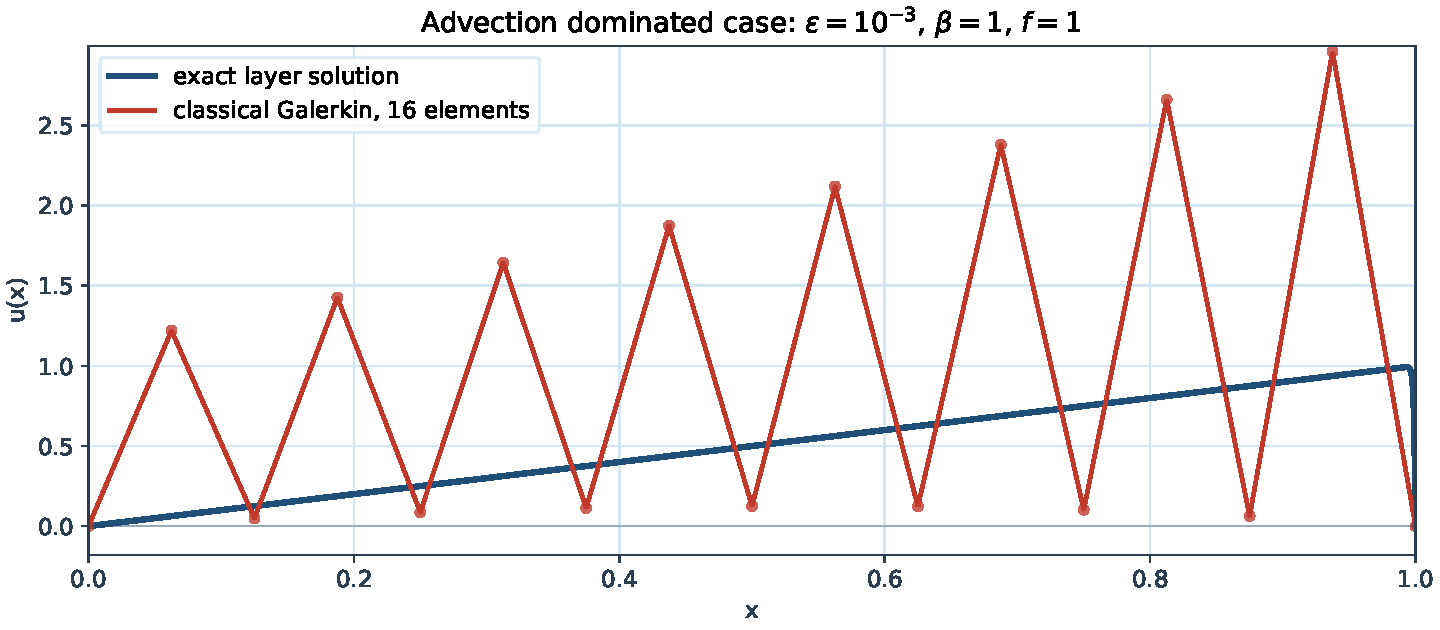
\includegraphics[width=0.88\linewidth]{figures/classical_oscillation.pdf}
\end{center}
\vspace{-0.25cm}
\softbox{Peach!45!PureWhite}{%
$u_1$ is an unstable approximation. We want some correction $u_B \in H_0^1(0,\ell)$ such that $u_1+u_B$ is a better approximation.}
\end{frame}

% ------------------------------------------------------------
\begin{frame}{4. Residual-free bubbles}
\accentbar
For a coarse approximation $u_1\in V_h^1$, define the element residual $r_K(u_1)=f-\mathcal{L}u_1$ with $\mathcal{L}w=-(\varepsilon w')'+\beta w'+\sigma w$. The ideal bubble correction on $K$ solves $\mathcal{L} \left(b_K \right) = r_K(u_1)$ in $K$ with  $(b_K)|_{\partial K}=0$.
\begin{center}
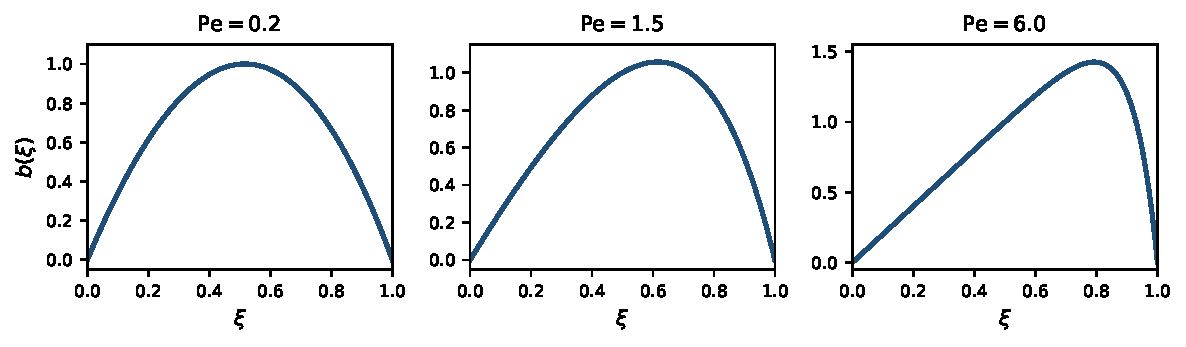
\includegraphics[width=0.6\linewidth]{figures/three_bubbles.pdf}
\end{center}
\softbox{Peach!45!PureWhite}{%
By construction $\mathcal{L}(u_1+b_K)=f$ on $K$: the ideal bubble exactly cancels the element residual. Enriching the space $V_h^1$ with these bubbles and solving the global Galerkin problem yields the RFB approximation $u_h = u_1 + \sum_K b_K$ \parencite{bubble_prompt, brezzi_rfb}.}
\end{frame}

% ------------------------------------------------------------
\begin{frame}{4. Residual-free bubbles}
\accentbar
\begin{center}
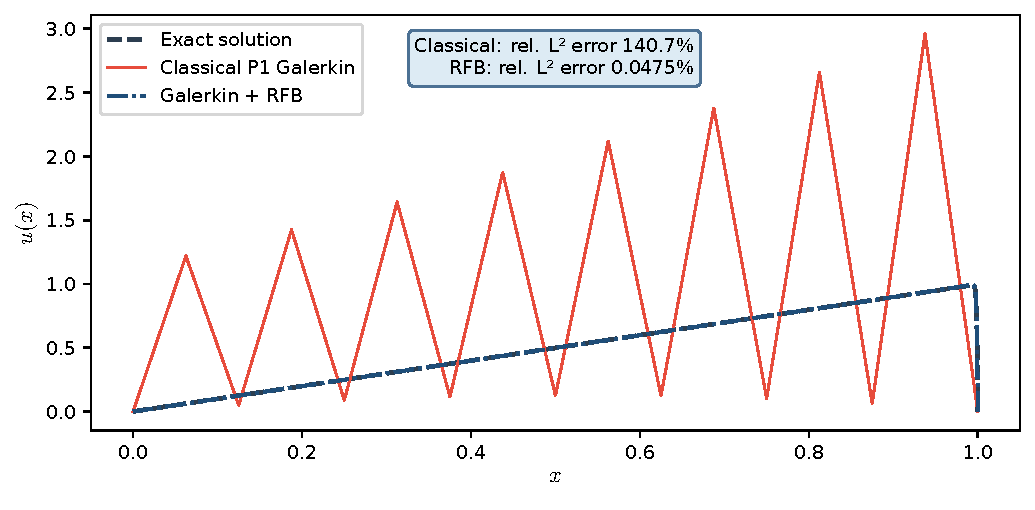
\includegraphics[width=0.8\linewidth]{figures/comparison_galerkin_rfb.pdf}
\end{center}
\vspace{-0.2cm}
\softbox{PastelBlue!40!PureWhite}{%
\small
With \textit{exact} bubbles the enriched space $V_h^1\oplus B$ contains the exact solution when $f$ is resolved by the bubble basis. Knowing the bubble map $u_1 \mapsto u_B $ is the key to making this approach practical without mesh refinement.}
\end{frame}

% ------------------------------------------------------------
\begin{frame}{5. The idea: learn the bubble functions}
\accentbar
{\color{Navy}\Large\bfseries Do not compute every bubble. Learn the bubble.}

\vspace{0.2cm}
\begin{columns}[T]
\begin{column}{0.47\linewidth}
\softbox{PastelBlue!40!PureWhite}{%
\textbf{Offline.} Solve many local RFB problems once to create training data.}
\end{column}
\begin{column}{0.47\linewidth}
\softbox{Peach!45!PureWhite}{%
\textbf{Online.} Evaluate the learned model from local parameters and statically condense the bubble.}
\end{column}
\end{columns}

\vspace{0.25cm}
\softbox{Mustard!32!PureWhite}{%
\textit{Learning} good $b_K$'s feeds the approximation $u_h = u_1 + \sum_K  b_{K}$, thus improving the overall solution.}
\end{frame}

% ------------------------------------------------------------
\begin{frame}{6. Data Generation ($ \varepsilon, \sigma, \beta \in \mathbb{R}^+ $)}
\accentbar
\small
We create a dataset $\mathcal{D}=\{(\mathbf{p}_i,\mathbf{y}_i)\}_{i=1}^N$ by solving the local bubble ODE on the reference element $[0,1]$:
\[
-\frac{\varepsilon}{h^2}b''+\frac{\beta}{h}b'+\sigma b = r(\xi),\quad b(0)=b(1)=0,\quad r\in\{1,\xi\}.
\]

\vspace{-0.15cm}
\begin{columns}[T]
\begin{column}{0.55\linewidth}
\softbox{PastelBlue!35!PureWhite}{%
\scriptsize
\textbf{Input $\mathbf{p}_i\in\mathbb{R}^2$}\qquad
$\displaystyle\Pe=\frac{\beta h}{2\varepsilon},\;
\rho=\frac{\sigma h^2}{\varepsilon}$
from physically relevant ranges of $(\varepsilon,\beta,\sigma)$.}
\vspace{0.06cm}
\softbox{Peach!40!PureWhite}{%
\scriptsize
\textbf{Target per mode $\mathbf{y}_i\in\mathbb{R}^{2Q}$}\qquad
For each mode $r\in\{1,\xi\}$ we store $(b(\xi_j),b'(\xi_j))_{j=1}^Q$ at Gauss points $\xi_j\in[0,1]$, where $b$ solves $\mathcal{L}_K b=r$ via finite differences.}
\end{column}
\begin{column}{0.42\linewidth}
\centering
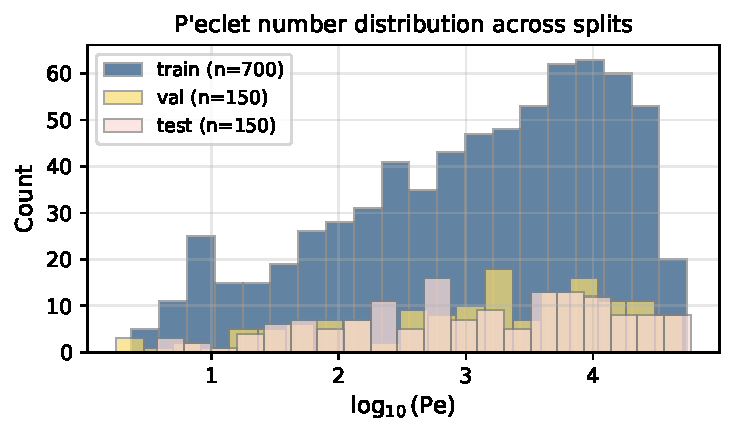
\includegraphics[width=0.85\linewidth]{figures/dataset_generation_fig.pdf}
\end{column}
\end{columns}
\end{frame}

% ------------------------------------------------------------
\begin{frame}{7. What is a \KAN{}?}
\accentbar

\vspace{-0.1cm}
\begin{center}
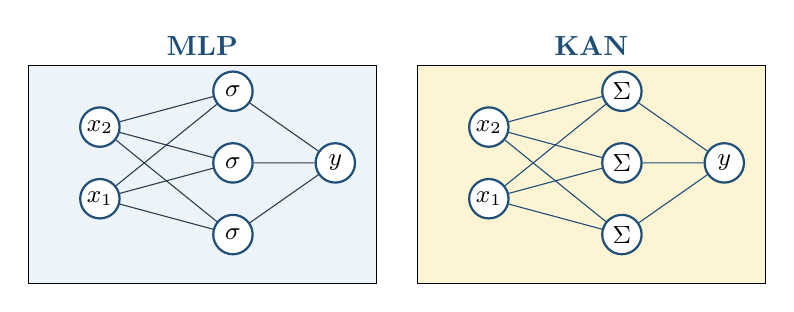
\begin{tikzpicture}[scale=0.65]
\definecolor{myblue}{HTML}{D4E6F1}
\definecolor{mymustard}{HTML}{F7DC6F}

% --- MLP network ---
\begin{scope}[xshift=-3.8cm]
  \draw[fill=myblue!45] (-1.8,-1.75) rectangle (5.0,2.5);
  \node[above, color=Navy, font=\bfseries] at (1.6,2.5) {MLP};
  \foreach \i/\lab in {0/$x_1$,1/$x_2$}
    \node[circle, draw=Navy, thick, fill=white, inner sep=0pt, minimum size=0.5cm] (m-in-\i) at (-0.4,\i*1.4-0.1) {\small\lab};
  \foreach \j in {0,1,2}
    \node[circle, draw=Navy, thick, fill=PureWhite, inner sep=0pt, minimum size=0.5cm] (m-hid-\j) at (2.2,\j*1.4-0.8) {\small$\sigma$};
  \node[circle, draw=Navy, thick, fill=white, inner sep=0pt, minimum size=0.5cm] (m-out) at (4.2,00.6) {\small$y$};
  \foreach \i in {0,1}
    \foreach \j in {0,1,2}
      \draw[Charcoal,thin] (m-in-\i) -- (m-hid-\j);
  \foreach \j in {0,1,2}
    \draw[Charcoal,thin] (m-hid-\j) -- (m-out);
  %\node[align=center, color=Charcoal] at (1.6,-1.55) {activation on nodes\\fixed $\sigma$, linear $w$};
\end{scope}

% --- KAN network ---
\begin{scope}[xshift=3.8cm]
  \draw[fill=mymustard!30] (-1.8,-1.75) rectangle (5.0,2.5);
  \node[above, color=Navy, font=\bfseries] at (1.6,2.5) {KAN};
  \foreach \i/\lab in {0/$x_1$,1/$x_2$}
    \node[circle, draw=Navy, thick, fill=white, inner sep=0pt, minimum size=0.5cm] (k-in-\i) at (-0.4,\i*1.4-0.1) {\small\lab};
  \foreach \j in {0,1,2}
    \node[circle, draw=Navy, thick, fill=PureWhite, inner sep=0pt, minimum size=0.5cm] (k-hid-\j) at (2.2,\j*1.4-0.8) {\small$\Sigma$};
  \node[circle, draw=Navy, thick, fill=white, inner sep=0pt, minimum size=0.5cm] (k-out) at (4.2,00.6) {\small$y$};
  \foreach \i in {0,1}
    \foreach \j in {0,1,2}
      \draw[Navy,thin] (k-in-\i) -- (k-hid-\j);
  \foreach \j in {0,1,2}
    \draw[Navy,thin] (k-hid-\j) -- (k-out);
  %\node[align=center,  color=Charcoal] at (1.6,-1.55) {\small activation on edges learnable $\phi$, sum $\Sigma$ on nodes};
\end{scope}
\end{tikzpicture}
\end{center}

\vspace{0.15cm}
\begin{columns}[T]
\begin{column}{0.48\linewidth}
\softbox{PastelBlue!40!PureWhite}{%
\small
\textbf{Key architectural difference}\\[2pt]
MLP: fixed nonlinearity on nodes, learnable linear scalars on edges.\\
KAN: learnable 1D functions (B-splines) on edges, summation on nodes.}
\end{column}
\begin{column}{0.48\linewidth}
\softbox{Peach!45!PureWhite}{%
\small
Each $\phi$ is a B-spline curve: smooth, compactly supported, and efficiently trainable. This gives (almost) the optimal $N^{-4}$ scaling law for cubic splines \parencite{kan_paper}.}
\end{column}
\end{columns}
\end{frame}

% ------------------------------------------------------------
% \begin{frame}[plain]
% \begin{tikzpicture}[remember picture,overlay]
%   \node[inner sep=0pt] at (current page.center)
%     {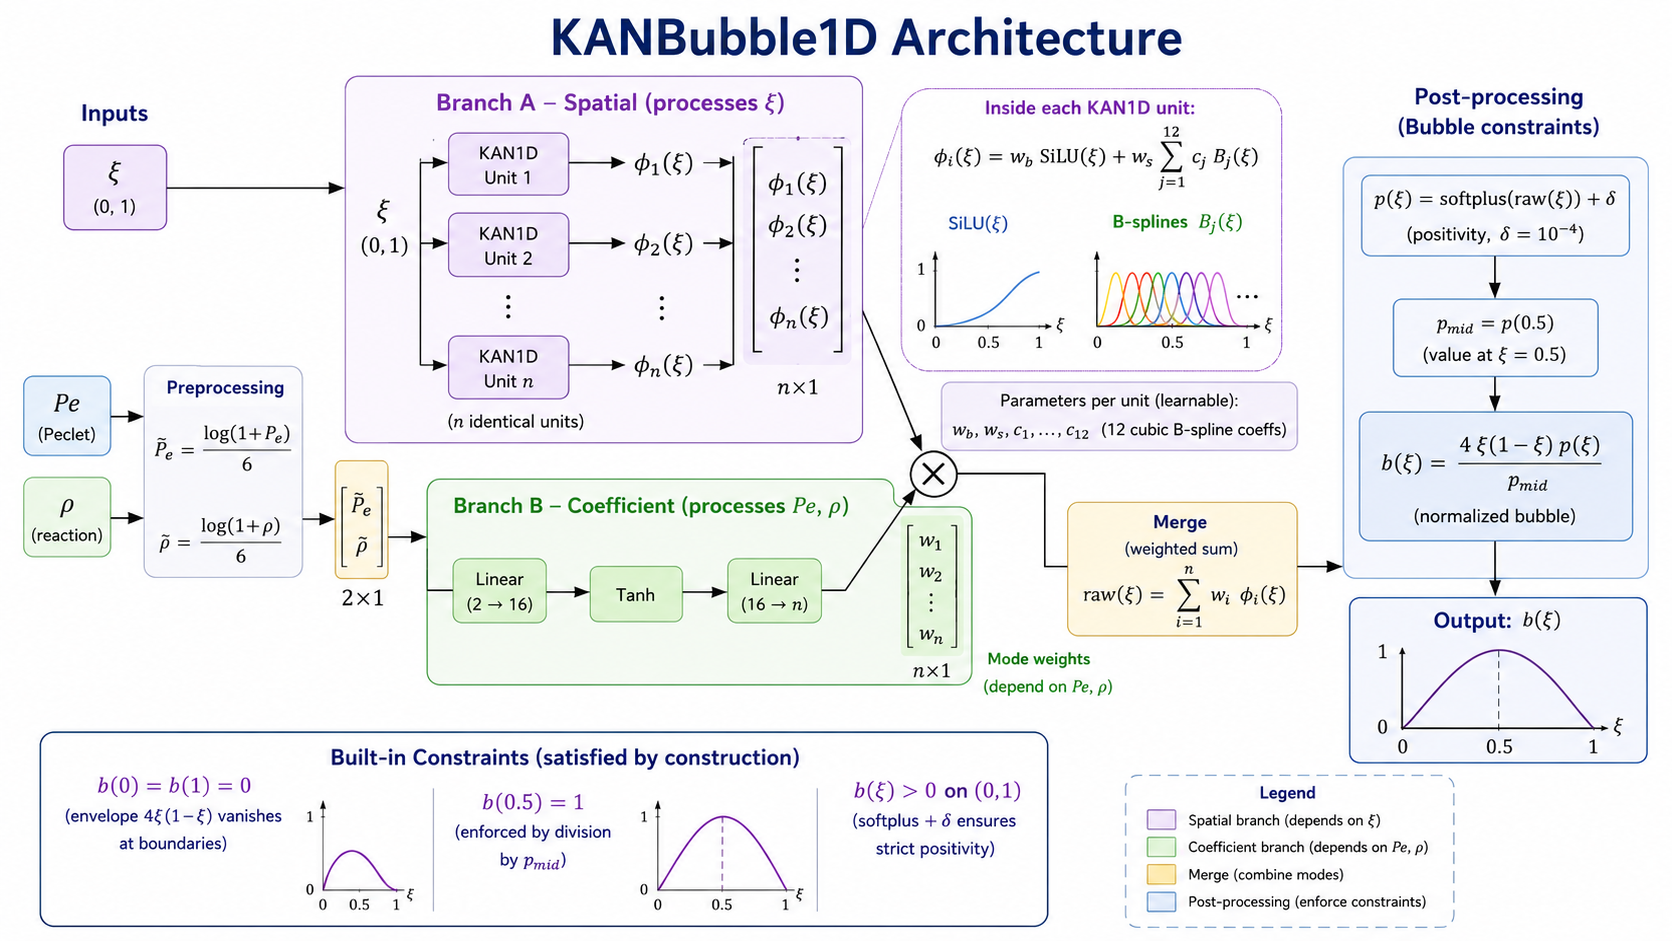
\includegraphics[width=\paperwidth,height=\paperheight,keepaspectratio]{figures/achitecture_figure_KAN1dBubble.png}};
% \end{tikzpicture}
% \end{frame}

% ------------------------------------------------------------
\begin{frame}{8. Learning bubbles with a \KAN{}}
\accentbar
We train a compact model that maps local parameters $(\Pe,\rho)$ to the bubble shape $b(\xi)$ for each mode $r\in\{1,\xi\}$, minimizing
\[
\mathcal{J}(\theta)=\|b_\theta-b^{\mathrm{RFB}}\|_{L^2 (0,1)}^2 +\eta\|b_\theta'-(b^{\mathrm{RFB}})'\|_{L^2 (0,1)}^2,
\]
where $b^{\mathrm{RFB}}$ is the reference FD solution.

\begin{columns}[T]
\begin{column}{0.48\linewidth}
\softbox{PastelBlue!40!PureWhite}{%
\textbf{What a \KAN{} gives us}
\begin{itemize}
    \item Smooth trainable 1D functions on edges.
    \item Compact representation of the parameter-to-shape map.
    \item Interpretable local nonlinear transformations.
\end{itemize}}
\end{column}
\begin{column}{0.48\linewidth}
\softbox{Peach!45!PureWhite}{%
\textbf{Why not a generic black box?}
\begin{itemize}
    \item The bubble is a structured local function.
    \item We want a compact model, not a huge network.
    \item Built-in constraints such as zero boundary values.
\end{itemize}
\vspace{0.1cm}
{\scriptsize \parencite{kan_paper, murphy_ml}}}
\end{column}
\end{columns}
\end{frame}

% ------------------------------------------------------------
\begin{frame}{9. Advantages of the process}
\accentbar
\vspace{0.1cm}
\softbox{PastelBlue!35!PureWhite}{%
\begin{itemize}
    \item Variational structure preserved, static condensation eliminates bubble DOFs locally.
    \item Global system size and sparsity pattern unchanged, same number of unknowns as $P_1-$Galerkin, same connectivity.
    \item Bubble learned on the reference element with dimensionless inputs $(\Pe,\rho)$; $h$ enters only through these numbers.
    \item Model trained once offline, reusable for any mesh $h$ without retraining.
    \item Naturally adapts to heterogeneous problems: $(\Pe,\rho)$ computed per element at assembly.
\end{itemize}}
\end{frame}

% ------------------------------------------------------------
\begin{frame}[allowframebreaks]{References}
\accentbar
\footnotesize
\printbibliography
\end{frame}

% ------------------------------------------------------------
\begin{frame}[plain]
\begin{tikzpicture}[remember picture,overlay]
  \fill[PastelBlue] (current page.south west) rectangle (current page.north east);
  \fill[PureWhite] ([xshift=0.9cm,yshift=0.9cm]current page.south west) rectangle ([xshift=-0.9cm,yshift=-0.9cm]current page.north east);
  \fill[Peach] ([xshift=1.15cm,yshift=-1.15cm]current page.north west) rectangle ++(2.4cm,0.12cm);
  \fill[Mustard] ([xshift=3.75cm,yshift=-1.15cm]current page.north west) rectangle ++(1.0cm,0.12cm);
\end{tikzpicture}
\vspace{2.0cm}
\begin{center}
{\color{Navy}\bfseries\Huge Questions?}\par
\vspace{0.45cm}
{\color{Charcoal}\large Learning Residual-Free Bubbles}\par
\end{center}
\end{frame}

\end{document}
